This thesis project has involved the implementation and evaluation
of many different components required to create an end-to-end wheelchair
navigation assistance system.

\subsection{Evaluation of machine learning models on preliminary dataset}
%include speed
The YOLOv5, DeepLabv3, and Hybridnets models were tested on the preliminary
video-only Curtin driving dataset. As this dataset is unlabelled, the
models were evaluated in terms of speed and potential usage, rather than accuracy.

A frame of YOLOv5 evaluated on the preliminary dataset can be seen in \cref{fig:yolov5}.
This model identifies vehicles and pedestrians with high accuracy, with the confidence in
a prediction decreasing as the object moves further away from the camera.

\begin{figure}[H]
    \centering
    \includegraphics[width=0.65\linewidth]{images/yolov5s.png}
    \caption{YOLOv5s evaluated on the Curtin dataset}
    \label{fig:yolov5s}
\end{figure}

A frame of DeepLabv3 evaluated on the preliminary dataset can be seen in \cref{fig:yolov5}.
DeepLabv3 identifies pedestrians with a high level of accuracy. However, the vehicles in the
image are not accurately segmented. This is likely due to the lower occurrence of vehicles
in the MS COCO dataset, which was used to train the model.
To repurpose this model for the task of drivable area segmentation,
it would have to be retrained on a labelled driving dataset such as BDD100K or Cityscapes.

\begin{figure}[H]
    \centering
    \includegraphics[width=0.65\linewidth]{images/deeplab.png}
    \caption{DeepLabv3 evaluated on the Curtin dataset}
    \label{fig:deeplab}
\end{figure}

An example of Hybridnets drivable area segmentation can be seen in \cref{fig:hybridnets}.
This model accurately detects drivable areas outdoors when a path is uniform, however
has more difficulty identifying a drivable path for non-uniform surfaces such as paved brick.
This is likely due to problems with domain adaptation, as the Hybridnets model was trained on the
BDD100K dataset which primarily consists of bitumen roads.
Hybridnets does not identify drivable area consistently when indoors
but does work well in some cases.

\begin{figure}[H]
    \centering
    \begin{subfigure}{.48\textwidth}
        \centering
        \includegraphics[width=\linewidth]{images/hybridnets_outdoor.png}
        \caption{Outdoors}
    \end{subfigure}
    \quad
    \begin{subfigure}{.47\textwidth}
        \centering
        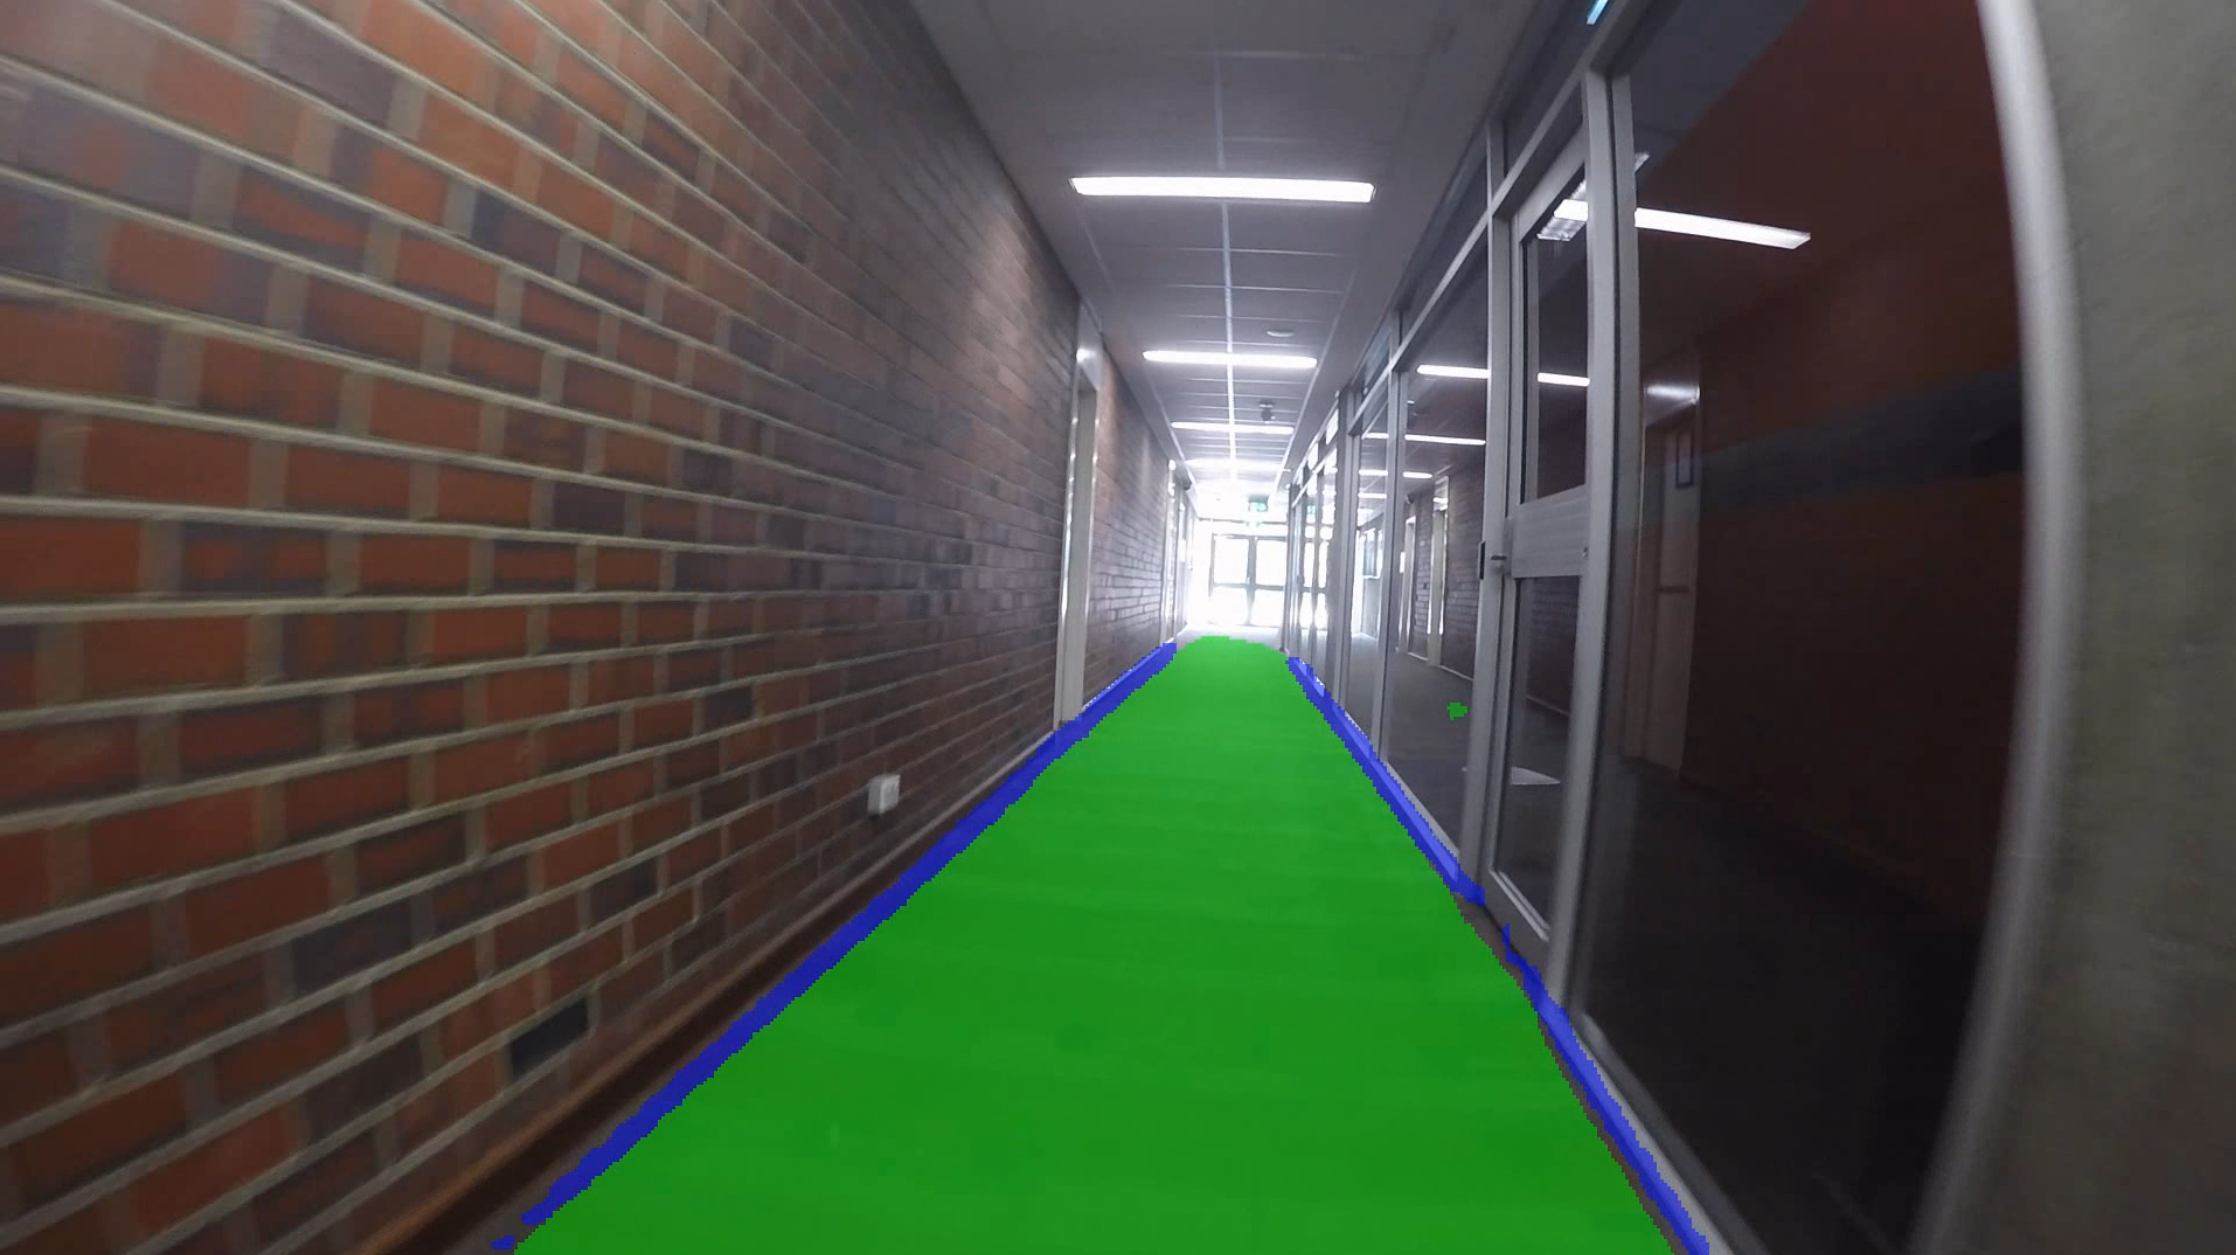
\includegraphics[width=\linewidth]{images/hybridnets_indoor.png}
        \caption{Indoors}
    \end{subfigure}
    \caption{Hybridnet drivable area segmentation evaluated on the Curtin dataset}
    \label{fig:hybridnets}
\end{figure}

The performance of each model (in frames per second) is given in \cref{table:model_fps}.
This performance was evaluated using a laptop with an RTX 3080 graphics card and AMD Ryzen 9 6900HX processor.
Note that Hybridnets is CPU limited, and could likely be optimized further by modifying postprocessing and video decoding methods.
Additionally,
Hybridnets runs both object detection and image segmentation using the same model.
YOLOv5 runs in real-time on our 24fps dataset, and can likely reach much higher speeds.

\begin{table}[H]
    \centering
    \begin{tabular}{c c c}
    \toprule
    Model Name & FPS & Notes \\
    \midrule
    YOLOv5 & Real-time & (Frame-rate of dataset was 24fps) \\
    DeepLabv3 & 21 &  \\
    Hybridnets & 10 & CPU limited (can likely be optimized) \\
    \bottomrule
    \end{tabular}
    \caption{Performance comparison of ML models}
    \label{table:model_fps}
\end{table}

\subsection{Hybridnets drivable area segmentation}
% do this first
In the last section, it was seen that the Hybridnets model generalised well in most cases,
however struggled with some non-uniform pathways such as paved brick.
The model was originally trained on the BDD100K dataset, which 

\pagebreak
\subsection{Efficiacy of birds-eye view occupancy map}
Once the drivable area has been segmented, it is transformed into the XZ plane
as a birds-eye view occupancy map. This is done by processing the 3D point cloud
data from the ZED Mini camera.
Morphological processing is used to improve the density of this occupancy map.
An example of the segmented output alongside the occupancy map can be seen in \cref{fig:occupancy_map_seg},
with the drivable area highlighted in green.
Note that the occupancy map is 15 metres long and 10 metres wide. The location of the ZED Mini camera is depicted
with an `X'; the camera is mounted to the right-hand side of the wheelchair.

\begin{figure}[b]
    % 16:6 width ratio
    % 0.64, 0.24
    \centering
    \begin{subfigure}{.64\textwidth}
        \centering
        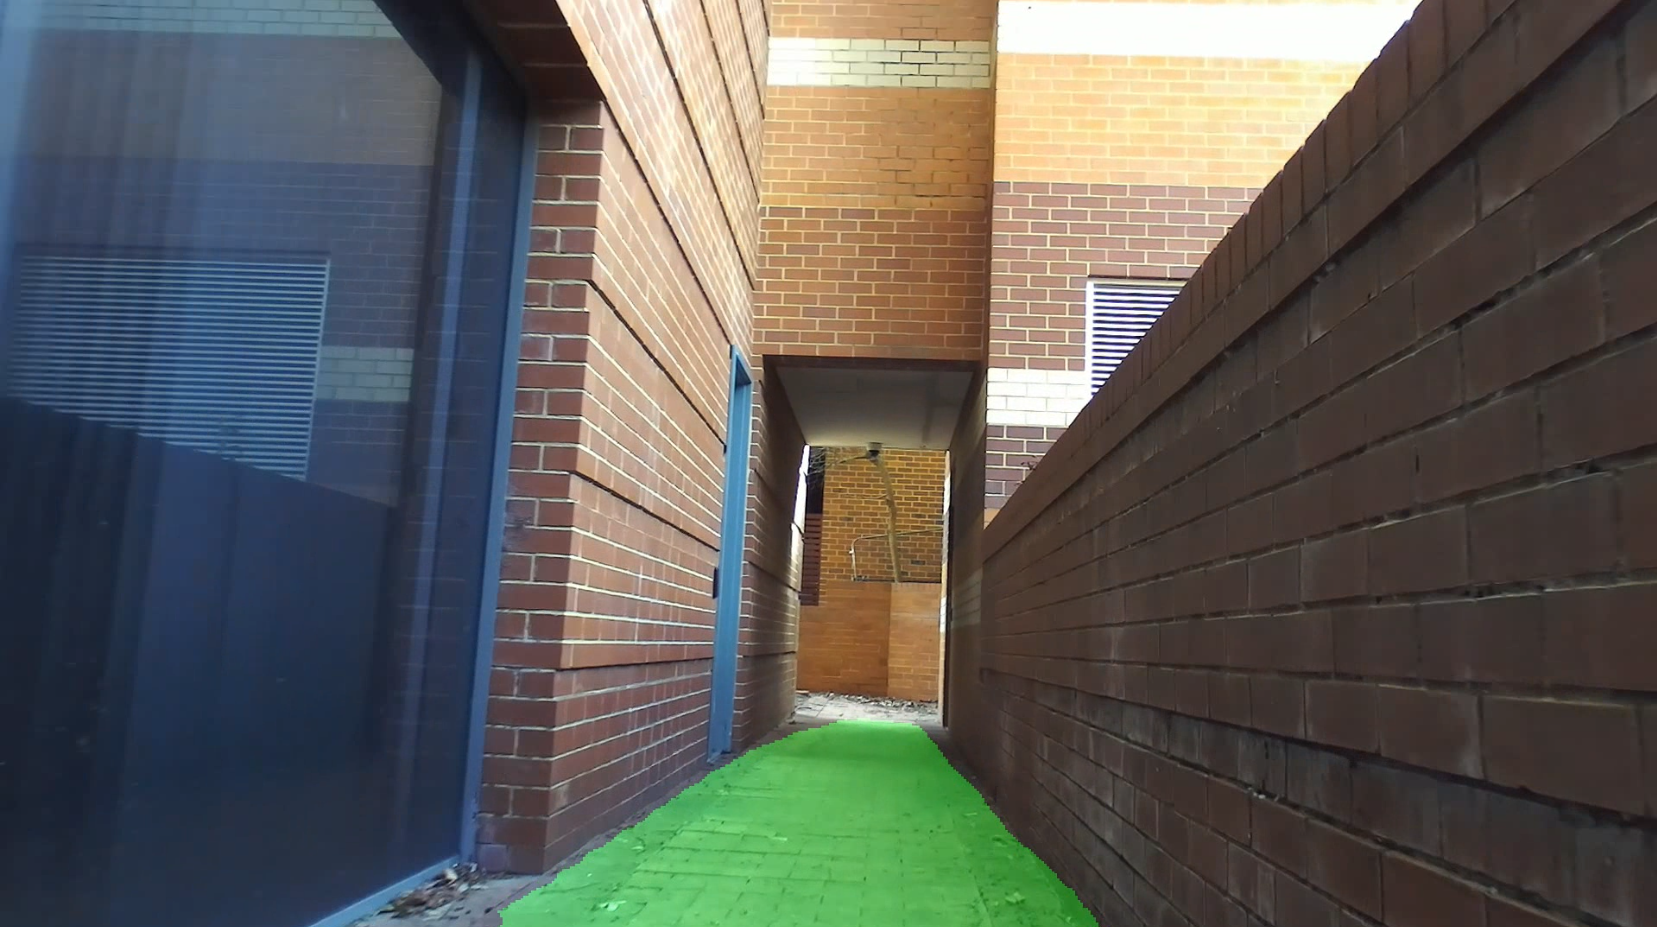
\includegraphics[width=\linewidth]{images/segmentation_1.PNG}
    \end{subfigure}
    \quad
    \begin{subfigure}{.24\textwidth}
        \centering
        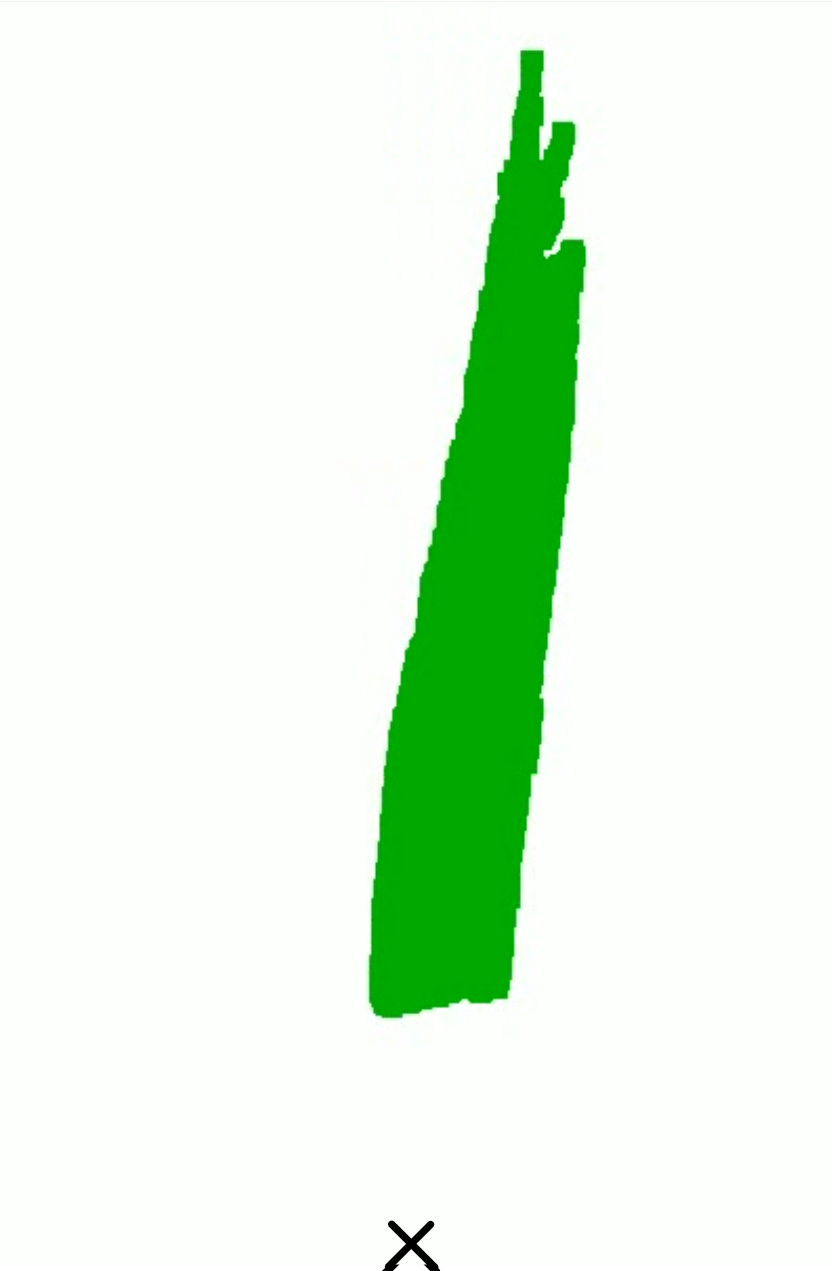
\includegraphics[width=\linewidth]{images/occupancy_map1.png}
    \end{subfigure}
    \begin{subfigure}{.64\textwidth}
        \centering
        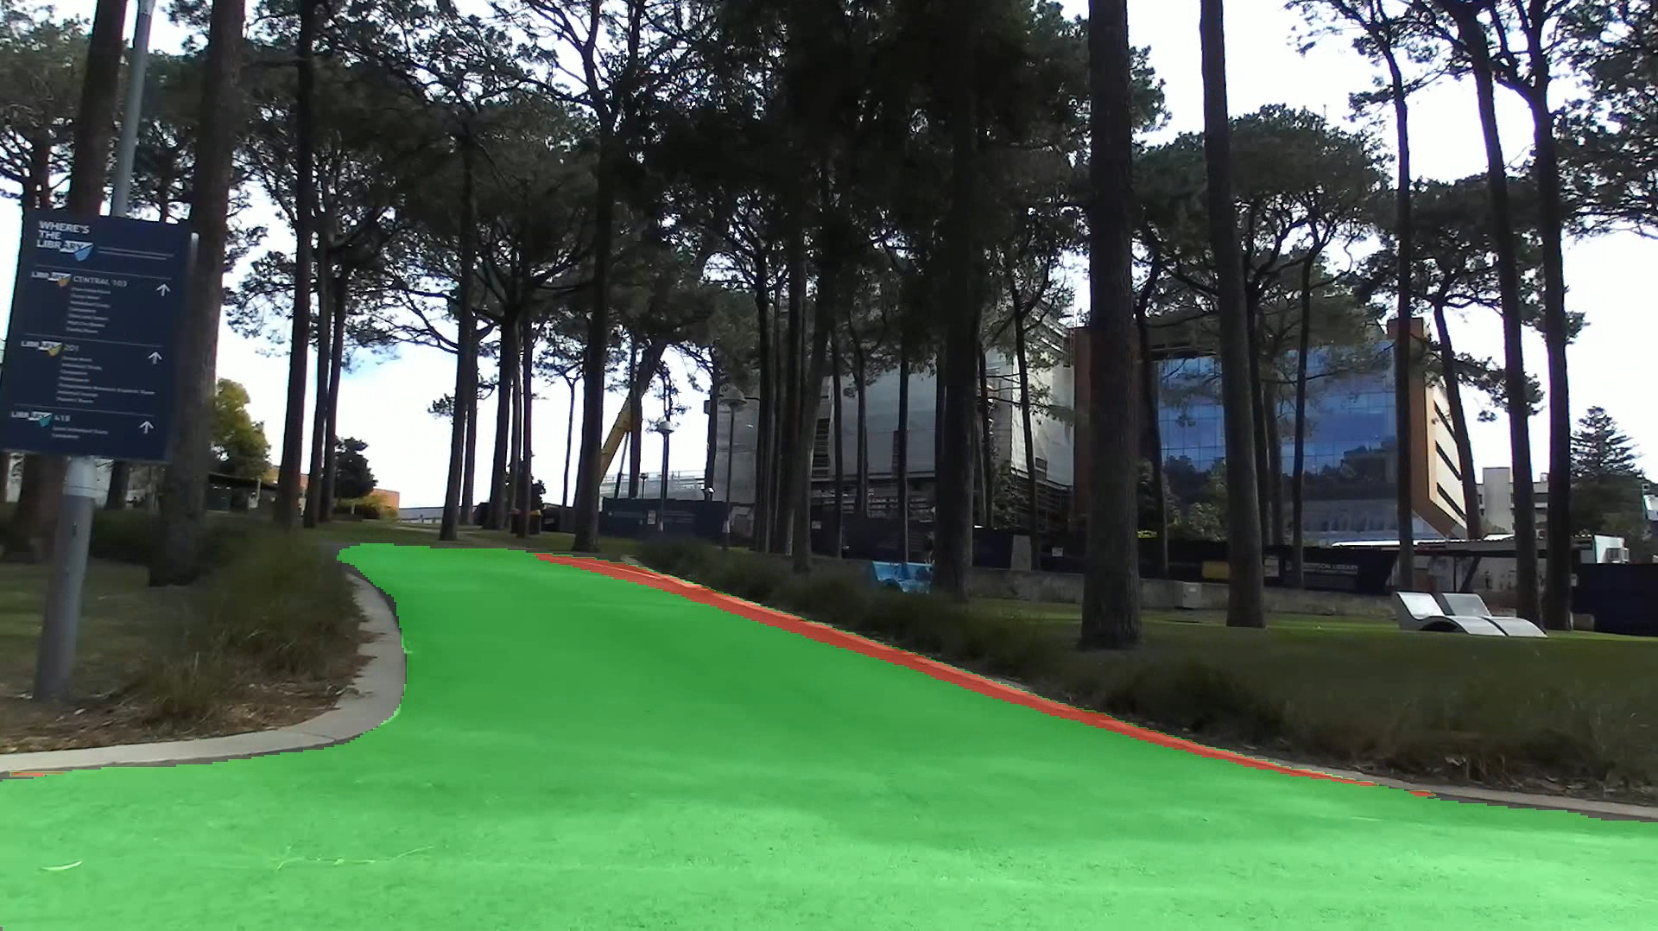
\includegraphics[width=\linewidth]{images/segmentation_2.PNG}
    \end{subfigure}
    \quad
    \begin{subfigure}{.24\textwidth}
        \centering
        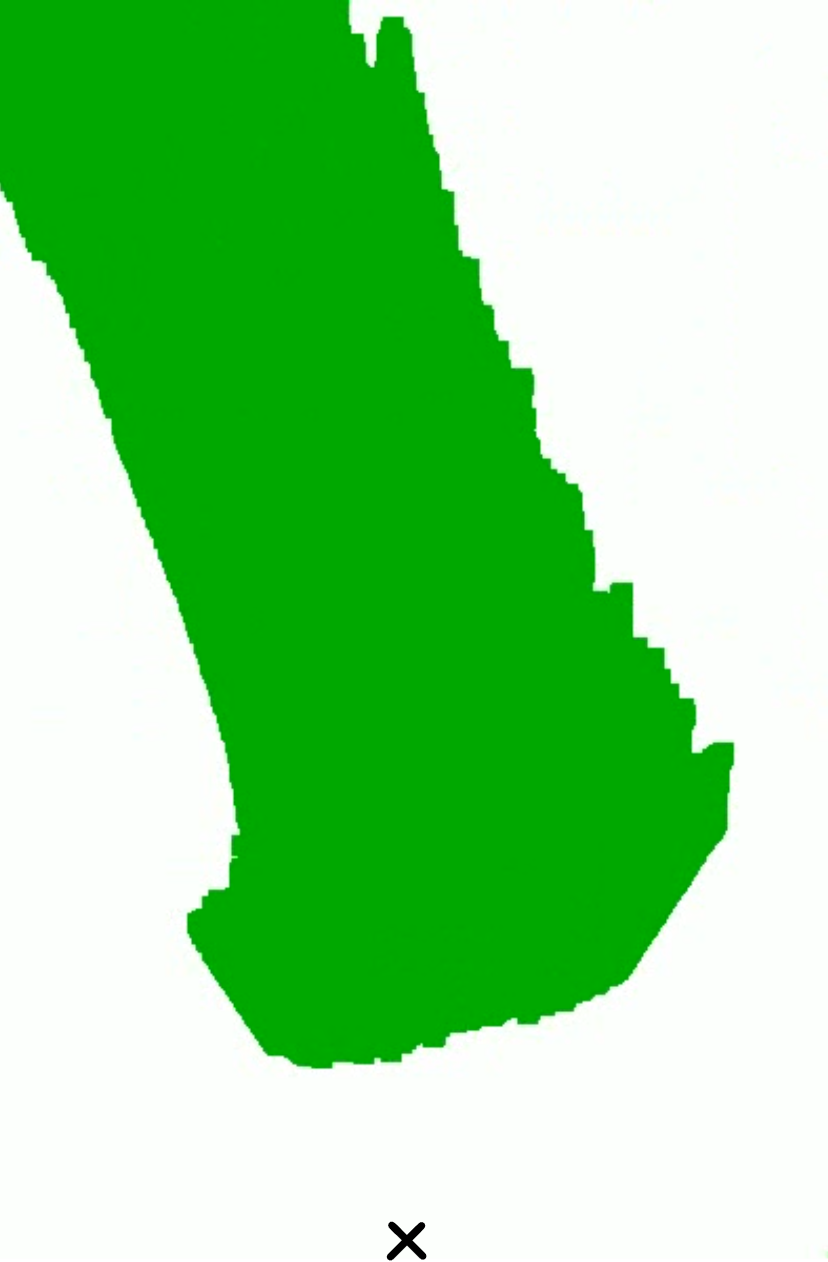
\includegraphics[width=\linewidth]{images/occupancy_map2.png}
    \end{subfigure}
    \begin{subfigure}{.64\textwidth}
        \centering
        \includegraphics[width=\linewidth]{images/segmentation_3.PNG}
    \end{subfigure}
    \quad
    \begin{subfigure}{.24\textwidth}
        \centering
        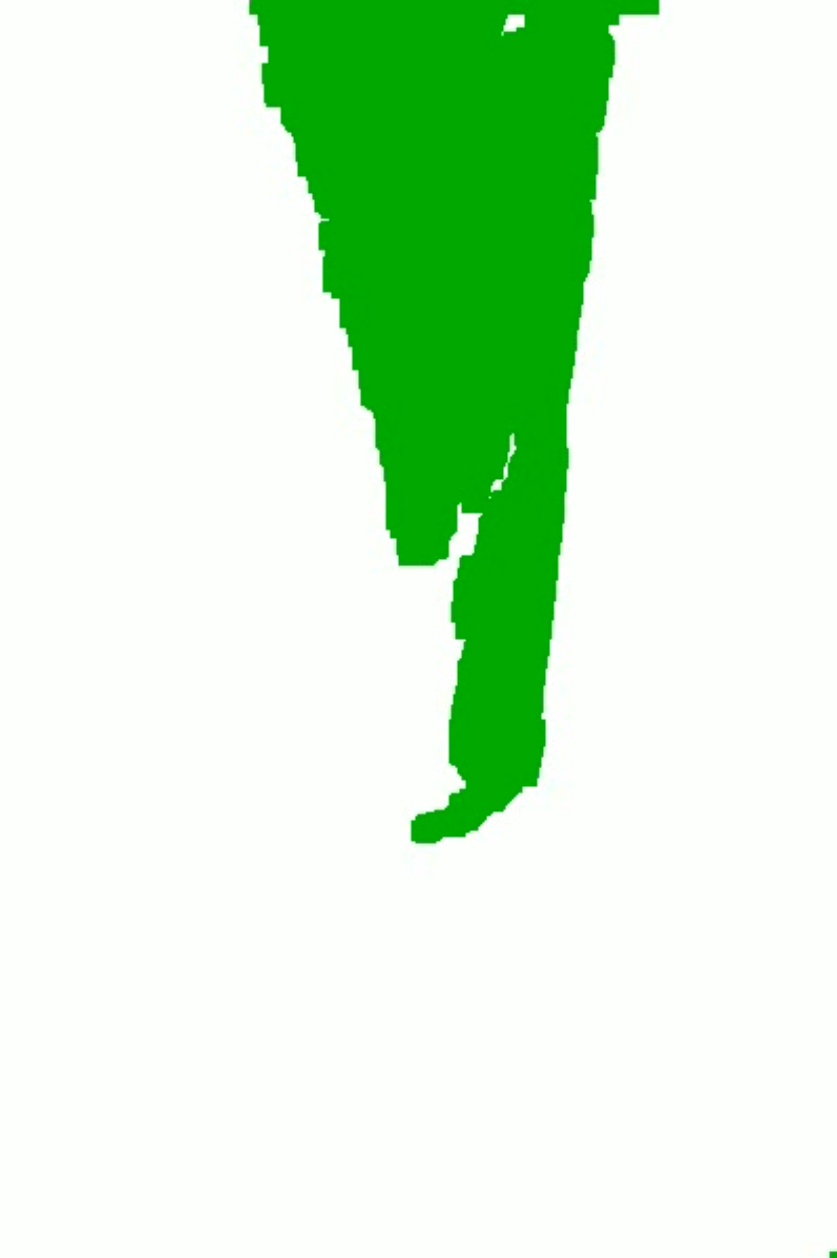
\includegraphics[width=\linewidth]{images/occupancy_map3.png}
    \end{subfigure}
    \caption{Segmented image output and corresponding occupancy map for three locations around Curtin university}
    \label{fig:occupancy_map_seg}
\end{figure}

This segmented image to occupancy map transform works well in all observed cases, as long as the Hybridnets model identifies the
drivable area accurately. One improvement that could be made to this implementation is its speed.
The algorithm is bottlenecked by the occupancy map transform code, which takes between \SI{150}{\milli\second}
and \SI{500}{\milli\second} to execute, depending on the size of the drivable area.

Although this approach reliably maps drivable areas to an occupancy grid,
the area directly in front of the wheelchair (approx. \SI{2.6}{\metre}) and behind the wheelchair is unknown due to the FOV of the camera.
Several approaches to rectify this are explored in \cref{sec:future_work}.

A comparison of the occupancy map before and after morphological processing is shown in \cref{fig:morphological_processing}.
Although the occupancy map has a higher resolution before this transformation, the poor density of the map
could make it more difficult to process. The time taken to perform this morphological processing is negligible
when compared to other sections of this code.

\begin{figure}[b]
    % 16:6 width ratio
    % 0.64, 0.24
    \centering
    \begin{subfigure}{.3\textwidth}
        \centering
        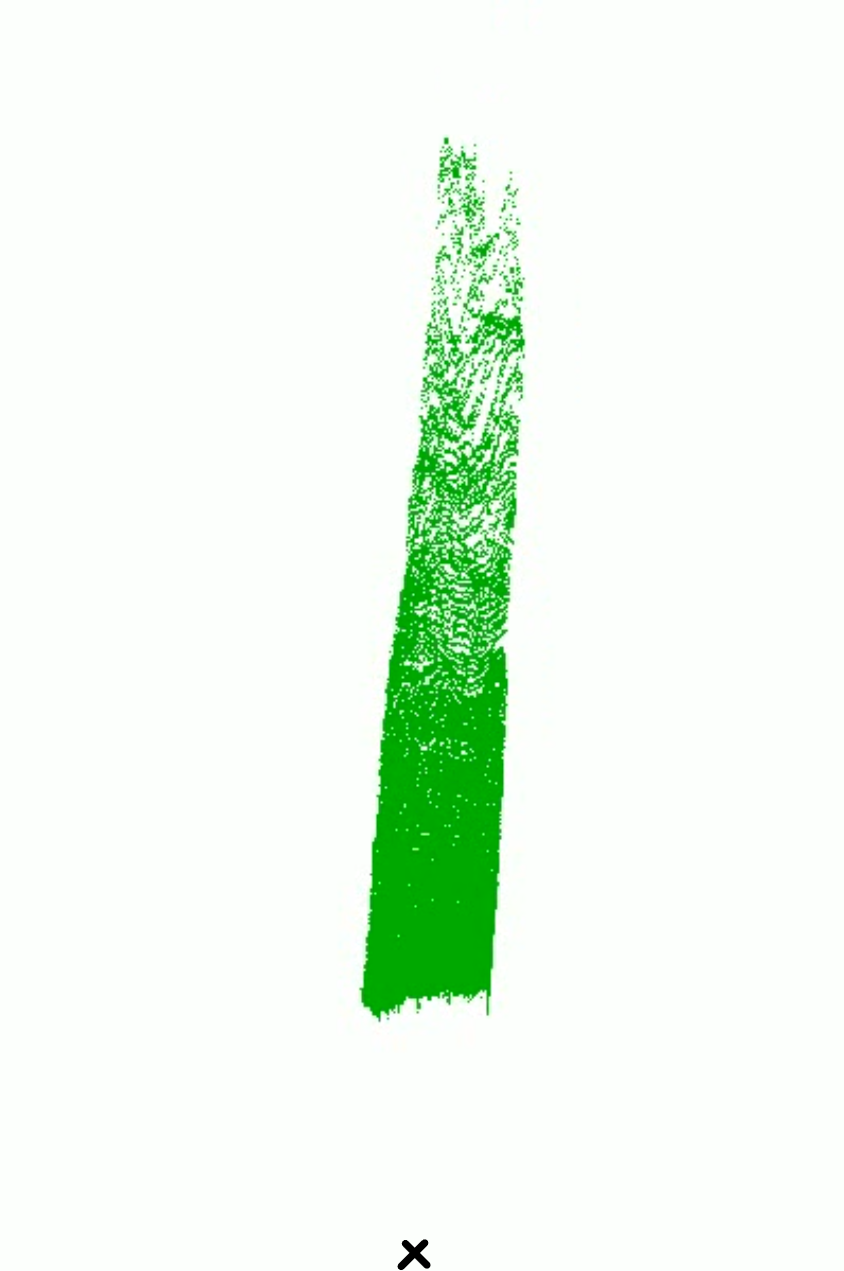
\includegraphics[width=\linewidth]{images/occupancy_map1_nomorph.png}
        \caption{Before processing}
    \end{subfigure}
    \quad
    \begin{subfigure}{.3\textwidth}
        \centering
        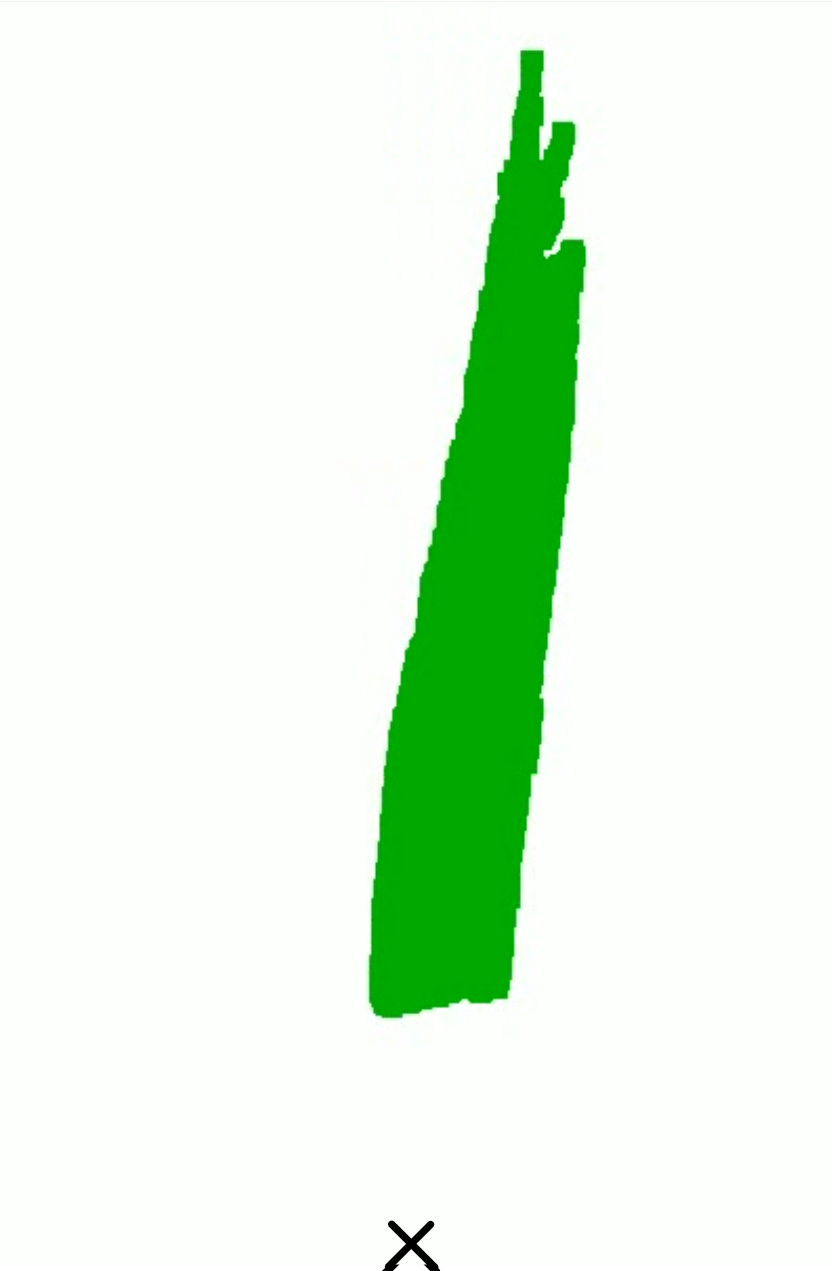
\includegraphics[width=\linewidth]{images/occupancy_map1.png}
    \end{subfigure}
    \caption{After processing}
    \label{fig:morphological_processing}
\end{figure}

\subsection{Evaluation of 3D point cloud obstacle detection algorithm}
% sensor tilt, find_floor_plane
% compare performance vs ultra depth mode


\subsection{Evaluation of assistive control algorithm}
% VFH+

\subsection{Evaluation of pose estimation APIs}
% positional tracking API
